\ifdefined\COMPILINGFROMMAIN
\else
    %%%%HEADER
\documentclass[twocolumn]{article}
\usepackage[a4paper, margin=1in, columnsep=20pt]{geometry}
\usepackage{amsmath, amssymb, graphicx, hyperref}
\usepackage[most,skins,breakable]{tcolorbox}
\usepackage[symbol]{footmisc}
\usetikzlibrary{calc}
\usepackage{xcolor}
\usepackage{caption}
\usepackage{algorithm}
\usepackage{algpseudocodex}
\usepackage{tikz}
\usepackage{listings}
\usetikzlibrary{arrows.meta, positioning}
\tcbuselibrary{listingsutf8}
\usepackage{microtype}
\usepackage{blindtext}
\usepackage{bookmark}
\usepackage{breqn}
\usepackage[backend=biber,style=numeric]{biblatex} % 
\addbibresource{../references.bib}

% Define style for the listings environment
\lstdefinestyle{mystyle}{
    basicstyle=\ttfamily\small,
    breaklines=true,
    escapeinside={(*@}{@*)}, % Allows math mode within listings
    numbers=left,
    numberstyle=\tiny,
    frame=single,
    keywordstyle=\color{blue}\bfseries,
    commentstyle=\color{green!50!black},
    stringstyle=\color{red}
}


\def\reals{\mathbb{R}}
% Define the custom definition box and command
\newtcolorbox{mydefinition}[2][]{%
    text width=0.95\columnwidth,
    before=\vspace{1mm}, 
    after=\vspace{1mm}, 
    colback=gray!10, % Background color (light gray)
    colframe=black!70,  % Border color
    coltitle=gray!10,  % Title color
    fonttitle=\bfseries, % Title font style
    sharp corners,   % Box style
    left=2pt,
    breakable,
    right=2pt,
    top=2pt,
    bottom=2pt,
    enhanced jigsaw,
    title=Definition: {#1},         % Title passed as the first argument
    colupper=black,  % Ensure proper content handling
    pad at break*=1pc,
    overlay first and middle={
        \coordinate (A1) at ($(interior.south east) + (-10pt,5pt)$);
        \coordinate (C1) at ($(interior.south east) + (-6pt,7.5pt)$);
        \draw[fill=black!50] (A1) -- +(0,5pt) -- (C1) -- cycle;
    }
    }
    
\newcommand{\definition}[2]{%
    \noindent%
    \begin{mydefinition}[#1]%
        .#2%
    \end{mydefinition}%
    \noindent
}

\newtcolorbox{myexample}[2][]{%
    text width=0.95\columnwidth,
    before=\vspace{1mm}, 
    after=\vspace{1mm}, 
    colback=orange!3, % Background color (light gray)
    colframe=black!70,  % Border color
    coltitle=gray!10,  % Title color
    fonttitle=\bfseries, % Title font style
    sharp corners,   % Box style
    left=2pt,
    right=2pt,
    top=2pt,
    bottom=2pt,
    breakable,
    title=Intuition: {#1},         % Title passed as the first argument
    pad at break*=1pc,
    overlay first and middle={
        \coordinate (A1) at ($(interior.south east) + (-10pt,5pt)$);
        \coordinate (C1) at ($(interior.south east) + (-6pt,7.5pt)$);
        \draw[fill=black!50] (A1) -- +(0,5pt) -- (C1) -- cycle;
    }
}

\newcommand{\example}[2]{%
    \noindent%
    \begin{myexample}[#1]%
    .#2%
    \end{myexample}%
    \noindent
}

\newtcolorbox{algobox}[2][]{%
    text width=0.95\columnwidth,
    before=\vspace{1mm}, 
    after=\vspace{1mm}, 
    colback=blue!5, % Background color (light gray)
    colframe=black!70,  % Border color
    coltitle=gray!10,  % Title color
    fonttitle=\bfseries, % Title font style
    sharp corners,   % Box style
    left=2pt,
    right=2pt,
    top=2pt,
    bottom=2pt,
    breakable,
    title=Algorithm: {#1},         % Title passed as the first argument
    pad at break*=1pc,
    overlay first and middle={
        \coordinate (A1) at ($(interior.south east) + (-10pt,5pt)$);
        \coordinate (C1) at ($(interior.south east) + (-6pt,7.5pt)$);
        \draw[fill=black!50] (A1) -- +(0,5pt) -- (C1) -- cycle;
    }
}

\newcommand{\algorithmbox}[2]{%
\noindent%
    \begin{algobox}[#1]%
    .#2%
    \end{algobox}%
    \noindent
}
%%%%HEADER

    \begin{document}
\fi
We will now describe a way to build an intrinsic triangulation of a Riemannian 2-Manifold $\big(\mathcal{M}, g\big)$, which enables the use of tools from Discrete Exterior Calculus, the cotan-Laplacian in which we are most interested in here. An intrinsic triangulation represents the intrinsic geometry - not an embedding of $\mathcal{M}$ into some ambient space. This is emphasized by the fact that we will be working with vertex coordinates in 2 dimensions, and will be interested in the edge-lengths under $g$, not the Euclidean distances between the vertices.
\\
\subsection*{Computing Edge Lengths through the Coordinate Space} 
Let the metric $g : C \to \reals^{2\times2}$. We will be triangulating the local-coordinate domain $C\subset \reals^2$ of the metric $g$, but using $g$ to measure the properties (lengths, areas) of the triangles. The triangulation will be an intrinsic triangulation of the manifold by encoding the metric in the edges and therefore having no notion of ambient space.
\\
In the introduction we have given the general formula for computing lengths of paths under the metric $g$. We will here consider the edges of the mesh as paths, and compute their length using this same formula. 
\\
For an edge $E = (A, B)$, we will parametrize it as $$r_i(t) = (1-t)A + tB$$ for $t\in[0,1]$. The measured length along the edge from $A$ to $B$, $e_i = m(A, B)$ is then computed as
\begin{align*}
    m(A, B) &:= \int_{0}^{1}\! \sqrt{\nabla r_i(t)^\top g(r_i(t)) \nabla r_i(t)} \, dt
    \\ 
    &= \int_{0}^{1}\! \sqrt{(B\!-\!A)^\top g(r_i(t)) (B\!-\!A)} \, dt
\end{align*}
By abbreviating the integrand as $$f(t) = \sqrt{(B\!-\!A)^\top g(r_i(t)) (B\!-\!A)}$$ we can get a simple formula for a numerical approximation using the trapezoidal rule:
\begin{align*}
    m(A, B) &= \int_{0}^{1}\! f(t) \, dt 
    \\
    &\approx \frac{1}{n\!+\!1}\!\left(\frac{f(0)\!+\!f(1)}{2} +  \sum_{t=1}^{n-1} f\!\left(\frac{t}{n\!+\!1}\right)  \right) 
\end{align*}
The trapezoidal rule is parametrized by the number of steps $n$ to take. The more steps, the more accurate the approximation.

\subsection*{What's the Catch?}
If we naïvely start applying this to a mesh overlaid onto the local coordinate system $C$, we might think that all is good and that we will have built a nice triangulation. However, if our mesh is not dense enough with respect to the rate of change of $g$, we might end up with \textit{Non-Planar} triangles.
\definition{Non-Planarity}{
    A key property of intrinsic triangulations are that each triangle can be locally embedded into a nonempty subset of $\reals^2$. This is enforced by the strict triangle inequality, which states that any two edges together are longer than the third edge, and that all edges are of nonzero length. 
    When a triangle does not satisfy the strict triangle inequality but has positive lengths, we will here refer to it as non-planar, because it cannot be embedded into the plane. The ratio of the longest edge to the shortest edge in a planar triangle will always be in the interval $(1, 2)$.
}
So? Well, for starters, Heron's formula (\ref{eq:heron}) for the area of a triangle will yield imaginary areas for non-planar triangles\footnote{This is how the author bumped into the concept in the first place and had to think about all of this.}. The operators of discrete exterior calculus will thus not be well-defined, and we will not be able to compute the Laplacian.
\\
In Euclidean space, all measurements along straight lines between three points $(A, B, C)$ in will result in planar triangles\footnote{If $(A, B, C)$ are collinear, the area of the triangle will be zero, but the standard triangle inequality is not violated.}. However, when we are measuring with the metric $g$ along straight line $(A \to B)$ in the $C$, we will generally not be taking the shortest path from $A$ to $B$ on the manifold. If the measured length $||AB||_g$ satisfies
$$||AB||_g > ||AC||_g + ||CB||_g$$
(which is \textit{the} violation of the triangle inequality), $A \to C \to B$ will be a shorter path. This is the essence of non-planarity, which motivates the need for the triangle inequality.
\\
To deal with non-planar triangles, one can subdivide them. There are many subdivision schemes of triangles, such as red-green refinement \cite{puppo2008rgbdivision}, butterfly subdivision \cite{dyn1990butterflydivision}, or the loop scheme \cite{loop1987smoothloopdivision}. We will use longest-edge bisection\cite{longest_edge_bisection}, which is simple to implement. When we repeatedly halve the longest edge of a non-planar triangle, the resulting triangles will eventually become planar, because any triangle can be made planar by shortening the longest edge enough.
\example{Fan Model}{
    To better understand the phenomenon of non-planarity, we suggest a mental model of the geometry encoded by the triangle in fig \ref{fig:non-planar-triangle} as part of a folded fan. The two shortest edges ($1, 1.5$) form the straight edges, while the longest one is scrunched up between them.
    \begin{center}    
        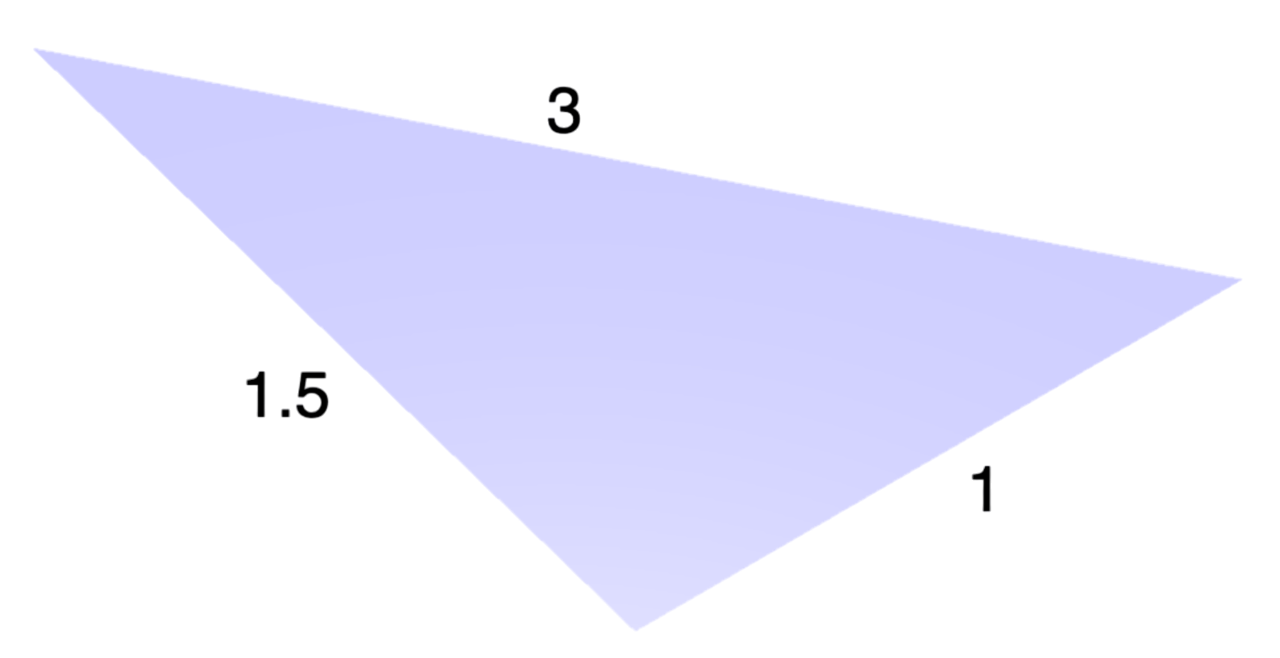
\includegraphics[width=0.9\columnwidth]{../images/cone_coordinate.png}
        \captionof{figure}{A non-planar triangle with edge lengths shown. Do not get fooled by the fact that it is being drawn in a plane - lengths are not to scale. The plane is merely the coordinate representation of the surface.}
        \label{fig:non-planar-triangle}
    \end{center}
    \begin{center}    
        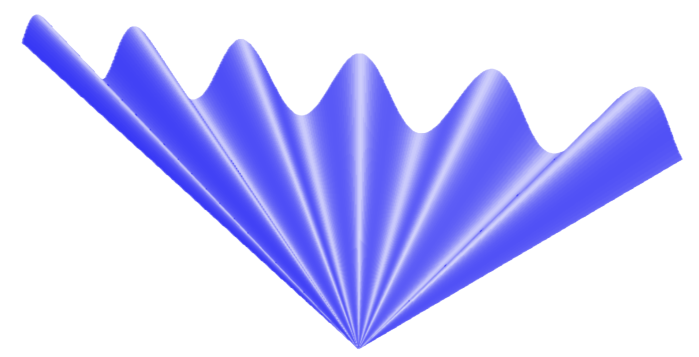
\includegraphics[width=0.8\columnwidth]{../images/fan.png}
        \captionof{figure}{A Euclidean embedding of the non-planar triangle requires curved geometry, as the triangle inequality is not satisfied. This figure shows one interpretation of a manifold that would result in the non-planar measurements.}\label{fig:fan_euclid}
    \end{center}
}
\example{Extrinsic vs Intrinsic Triangulation of the Fan model}{
    \begin{center}    
        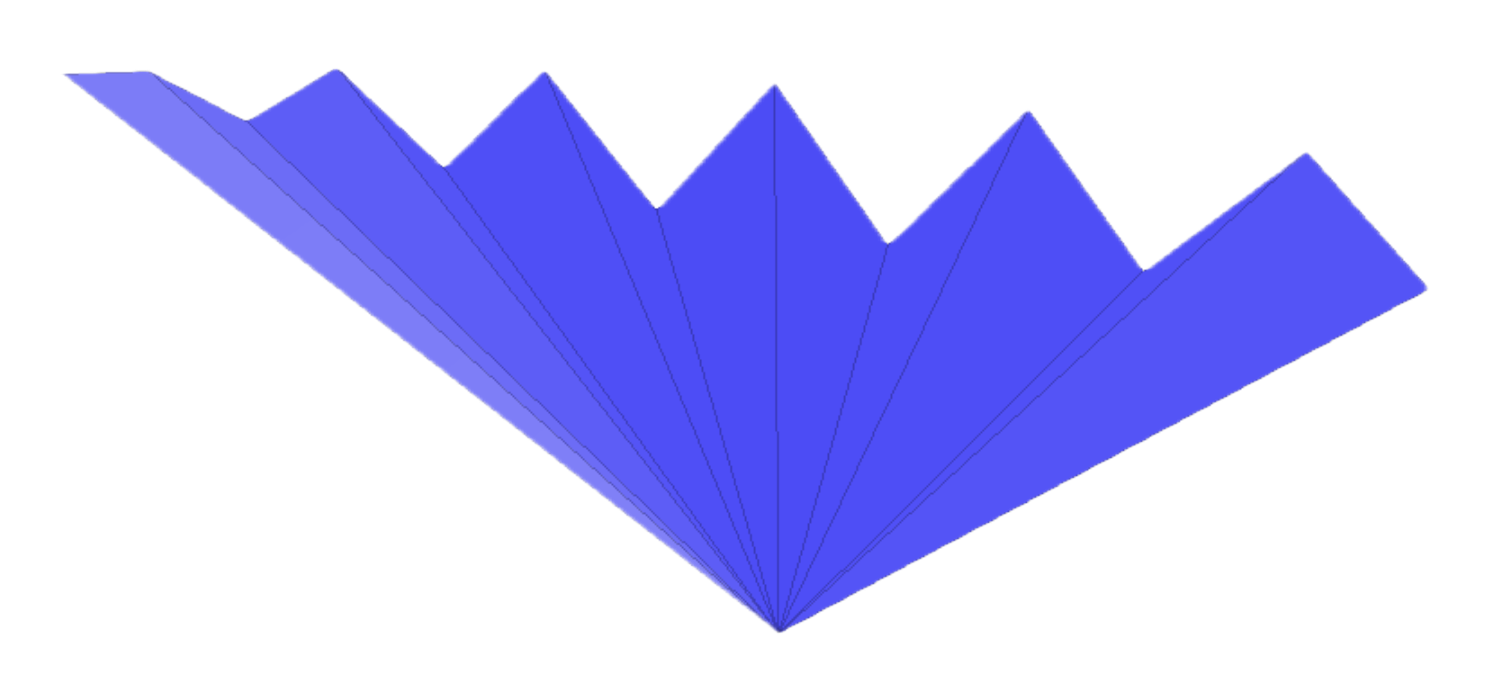
\includegraphics[width=0.8\columnwidth]{../images/fan_extrinsic.png}
        \captionof{figure}{An extrinsic 12-triangle isometrically embedded approximation of the fan model. The mesh stores only vertex positions. In ambient space, each vertex "sits" exactly on the manifold, while the planes spanned inbetween are linear approximations and will generally move away from the manifold.}
    \end{center}
    \begin{center}    
        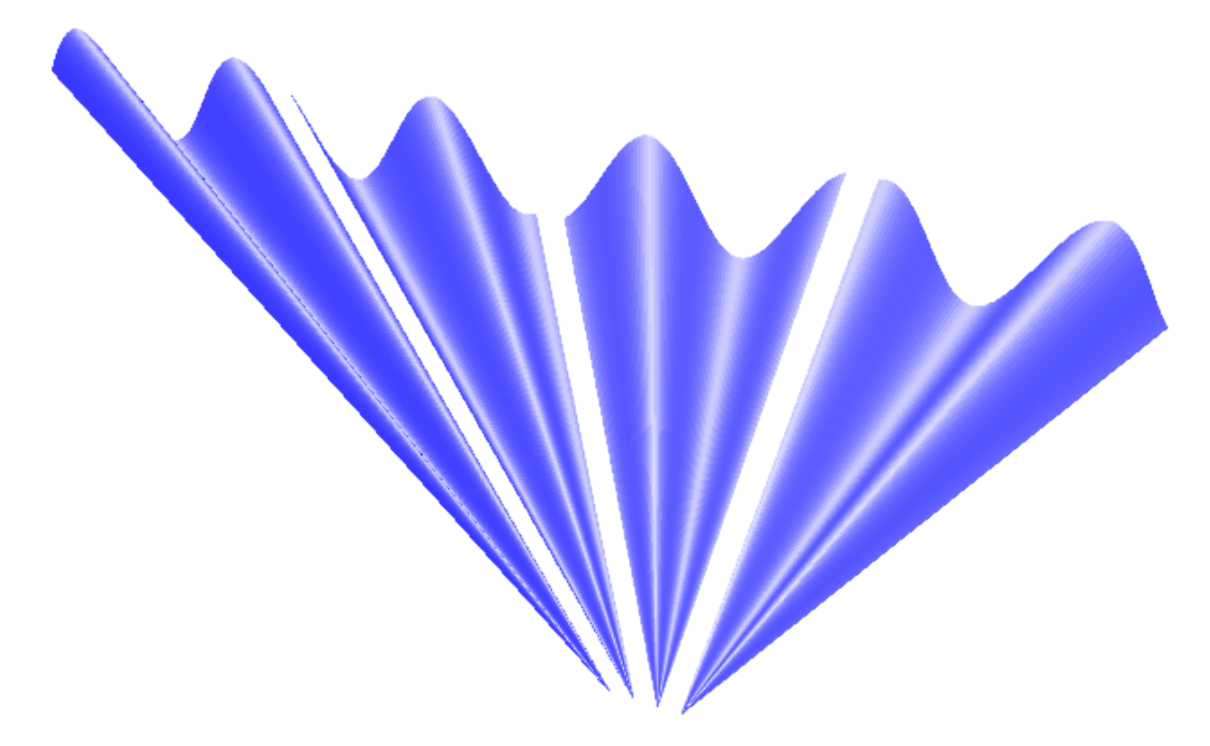
\includegraphics[width=0.8\columnwidth]{../images/fan_intrinsic.png}
        \captionof{figure}{An intrinsic 4-triangle representation of the fan model. The mesh stores edge-lengths only. We render the triangulation onto the Euclidean embedding (fig \ref{fig:fan_euclid}) to highlight the fact that edge-lengths are measured along the manifold, not in straight lines through ambient space. The manifold has been cut along the 3 interior edges of a 4-triangle mesh to show how it is implicitly partitioned.}
    \end{center}
}\noindent
We will now give our algorithm that builds the intrinsic triangulation. The algorithm is split into two phases: setup and refinement. The setup phase will compute the edge-lengths of the initial mesh and mark triangles that are non-planar, have edges that are too long or too short, or have an area that is too large. The refinement phase will then iteratively split the longest edge of the marked triangles and inspect the new triangles for the same properties. The algorithm will terminate after a fixed number of iterations or when there are no more marked triangles.
\algorithmbox{Setup Intrinsic Triangulation}{
    \textbf{Input:} $\vspace{3mm}$
    \\$M$ : Initial mesh that partitions the coordinate space $C$. $\vspace{1mm}$
    \\$g$ : Metric, mapping from any point in $C$ to 2x2 matrix.$\vspace{1mm}$
    \\$\rho$ : Desired maximal edge ratio in any triangle, $1 < \rho < 2$ $\vspace{1mm}$
    \\$A_{\text{max}}$ : Desired maximal area of any triangle.
    \\$\vspace{3mm}$%
     \textcolor[RGB]{170,170,170}{\rule{\linewidth}{0.4pt}}
    \transparent{0.5}%
    \textit{Step 1: Compute edge-lengths.} $\vspace{2mm}$
    \transparent{1.0}
    \\\textbf{for each} edge $E_i = (A, B)$ \textbf{in} $M$: $\vspace{2mm}$
    \begin{adjustwidth}{10px}{}
        Numerically compute the edge-length as \\$e_i = m(A, B)$\\
    \end{adjustwidth}
    \transparent{0.5}%
    \textit{Step 2: Inspect triangles.} $\vspace{2mm}$
    \transparent{1.0}
    \\Initialize \textbf{T} as the empty set $\vspace{2mm}$
    \\\textbf{for each} triangle $T$ \textbf{in} $M$: $\vspace{2mm}$
    \begin{adjustwidth}{10px}{}
        Add $T$ to \textbf{T} if
        \begin{adjustwidth}{10px}{}
            the ratio $e_{\text{long}}/e_{\text{short}}$ exceeds $\rho$ or
            \\
            the area exceeds $A_{\text{max}}$
            \\$\vspace{-2mm}$%
        \end{adjustwidth}
    \end{adjustwidth}
    $\vspace{2mm}$%
     \textcolor[RGB]{170,170,170}{\rule{\linewidth}{0.4pt}}
    \\\textbf{Output:} $\vspace{2mm}$
    \\$\mathbf{\Delta}_0$ : Mesh $M$ with computed edge-lengths. $\vspace{1mm}$
    \\\textbf{T} : Set of marked triangles.
}\noindent
\\
For the subsequent refinement phase, it will be useful to have a figure to refer to that explains the naming.
\definition{Local Triangle Naming scheme}{For a given triangle, we refer to edges as $E_{\text{long}}, E_{\text{medium}}, E_{\text{short}}$ with the property $e_{\text{long}} \geq e_{\text{medium}} \geq e_{\text{short}}$. \\The vertex opposing $E_{\text{long}}$ edge is \underline{\textbf{C}}orner, the vertex on the shortest edge \underline{\textbf{S}}hort, and the remaining vertex on the medium-length edge \underline{\textbf{M}}edium. The vertex across $E_{\text{long}}$ in a potential adjacent triangle is \underline{\textbf{O}}pposite. \\In the figure below, let $T$=SMC be the reference triangle. We have $E_{\text{long}}$=SM, $E_{\text{medium}}$=CM, and $E_{\text{short}}$=CS.
\vspace{-5mm}\begin{center}    
    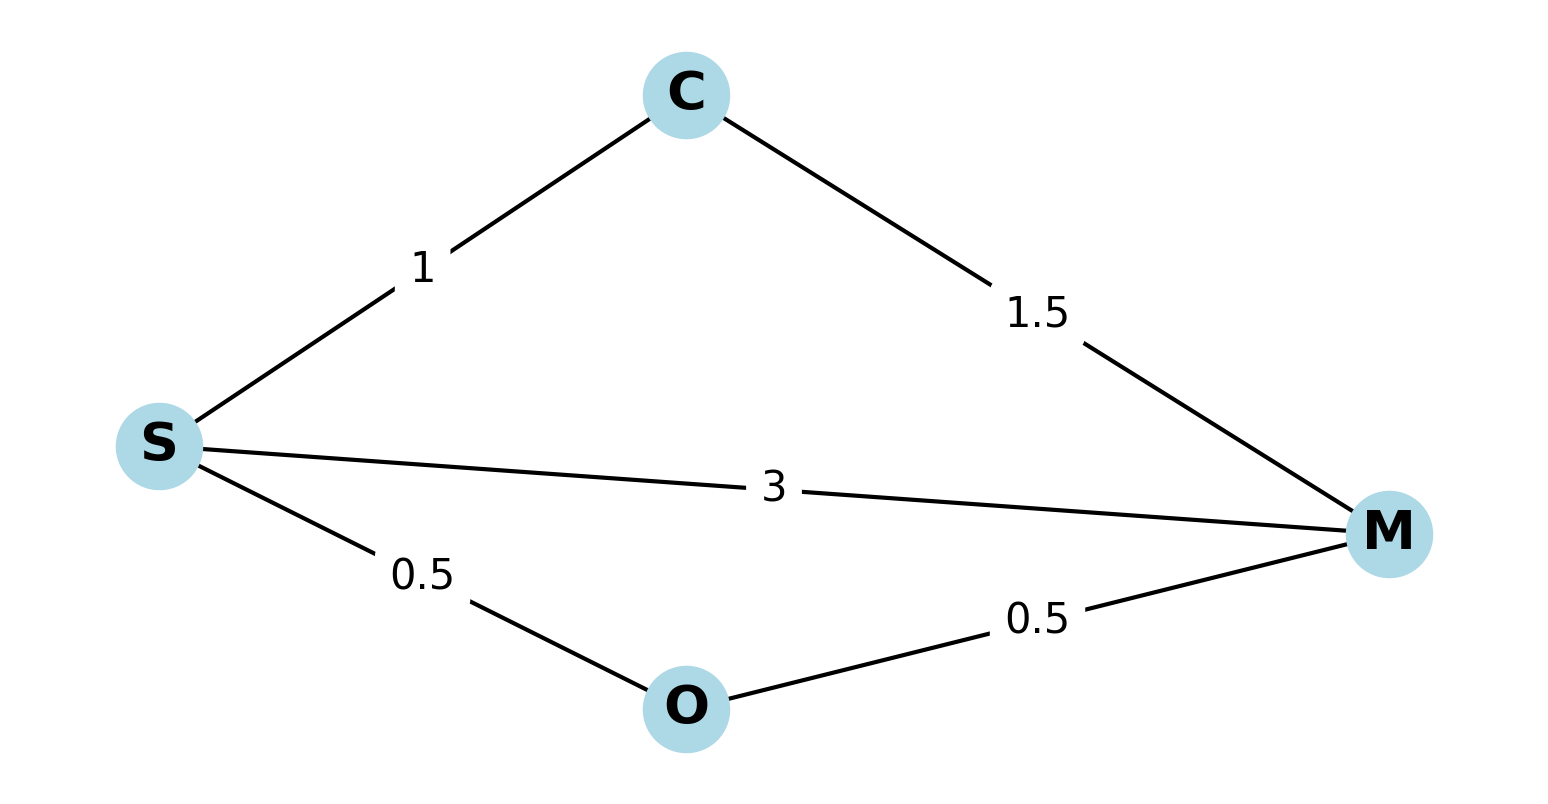
\includegraphics[width=1\columnwidth]{../images/mesh_refine_1.png}
    \captionof{figure}{The reference triangle patch illustrating  the naming scheme of the upcoming algorithms. This figure additionally serves as an example output $\mathbf{\Delta}_0$ of the setup phase. Both triangles would be in the output \textbf{T} due to their non-planarity.}
    \label{fig:naming_scheme}
\end{center}
}
\algorithmbox{Refine Intrinsic Triangulation}{
    \textbf{Input:} $\vspace{3mm}$
    \\$\mathbf{\Delta}_0$ : Initial intrinsic triangulation with edge-lengths. $\vspace{1mm}$
    \\\textbf{T} : Set of marked triangles.$\vspace{1mm}$
    \\$g$, $\rho$, $A_{\text{max}}$: As described in setup.$\vspace{1mm}$
    \\$\textbf{i}_{max}$ : Maximal number of subdivisions.
    \\$\vspace{3mm}$%
    \textcolor[RGB]{170,170,170}{\rule{\linewidth}{0.4pt}}
    \textbf{i} $\leftarrow$ 0$\vspace{2mm}$
    \\\textbf{while} \textbf{T} is not empty \textbf{and} \textbf{i} $<$ $\textbf{i}_{max}$:  $\vspace{2mm}$
    \begin{adjustwidth}{10px}{}            
            \textbf{i} $\leftarrow$ \textbf{i} + 1$\vspace{2mm}$
            \\
            Select the marked triangle $T=SMC\in\textbf{T}$ with the largest perimeter and remove $T$ from \textbf{T}.
            \\\\
            \transparent{0.5}%
            \textit{Step 1: Split longest edge.}$\vspace{2mm}$
            \transparent{1}
            \\
            Find Euclidean midpoint of longest edge $E_{\text{long}}$, define it as new vertex at $N$. $\vspace{2mm}$
            \\
            Remove previous edge $MS$, insert new edges $NS$, $MN$. $\vspace{2mm}$
            \\
            With metric $g$, compute $|NS| = m(N, S)$ and $|MN| = e_{\text{long}} - |NS|$$\vspace{2mm}$
            \\\\
            \transparent{0.5}%
            \textit{Step 2: Bisect faces.} $\vspace{2mm}$
            \transparent{1.0}
            \\
            Split $T$ and the adjacent triangular face $T^\prime$=SOM opposite $E_{\text{long}}$ to get triangles $SON$, $NOM$, $NMC$, $NCS$.$\vspace{2mm}$
            \\
            Remove $T^\prime$ from \textbf{T}. $\vspace{2mm}$ 
            \\
            Compute new edge-lengths $CN$ and $NO$: $|CN| = m(C, N)$, $|NO| = m(N, O)$. $\vspace{1mm}$$\vspace{2mm}$
            \\\\
            \transparent{0.5}%
            \textit{Step 3: Inspect new triangles.} $\vspace{2mm}$
            \transparent{1.0}
            \\
            Evaluate the area and aspect ratio of $SON$, $NOM$, $NMC$, and $NCS$. $\vspace{2mm}$
            \\
            Based on $\rho$, and $A_{\text{max}}$, mark triangles for refinement by adding them to \textbf{T}.
            \\$\vspace{-2mm}$%
    \end{adjustwidth}
    \textcolor[RGB]{170,170,170}{\rule{\linewidth}{0.4pt}}$\vspace{2mm}$\\
    \textbf{Output:} $\vspace{2mm}$
    \\
    $\mathbf{\Delta}$ : Refined Intrinsic Triangulation, everywhere satisyfing the triangle inequality\footnote{This is not the case if the max iterations have been set too low.}$\vspace{1mm}$
}\noindent
During subdivision, we are constructing an intrinsic partition of the manifold into triangles. A triangle might require multiple bisections before it becomes planar. Note that, before any splitting, we didn't have just a bad approximation - we had \textit{no} approximation. Splitting was necessary to work with the geometry.  
\newpage
\subsection*{Results}
\subsubsection*{Triangulating Gaussian Bump}
We define our own metric similarly to the hemisphere metric example in section \ref{sec:manifolds}.
The map $f$ from coordinate space $C = (-1, 1) \times (-1, 1)$ is given as 
$$f(\begin{pmatrix}
    x \\ y
\end{pmatrix}) = $$
$$\exp\left(-\left(\begin{pmatrix}
    x & y
\end{pmatrix} \begin{bmatrix} 0.1 & 0.1 \\ 0.1 & 0.35 \end{bmatrix}^{-\!1} \begin{pmatrix}
    x \\ y
\end{pmatrix}\right)^2\right)$$
Figure \ref{fig:bell_input} shows the initial coarse mesh. The algorithm is run for $500$ steps with $A_{\text{max}} = 1/8$ and $\rho = 1.2$. The output is shown in figures \ref{fig:bell_tissot}. The mesh is now more dense around the peak of the bump, where the curvature is higher. The mesh is not an embedding of the manifold, but an intrinsic triangulation. An embedding using $f$ is shown in fig \ref{fig:bell_embedded}, giving an extrinsic representation. We might not generally have access to $f$, and this figure is for illustration purposes only. Notice that triangles that appear very thin and stretched in the intrinsic triangulation are not so after being embedded isometrically.
\begin{figure}
    \centering
    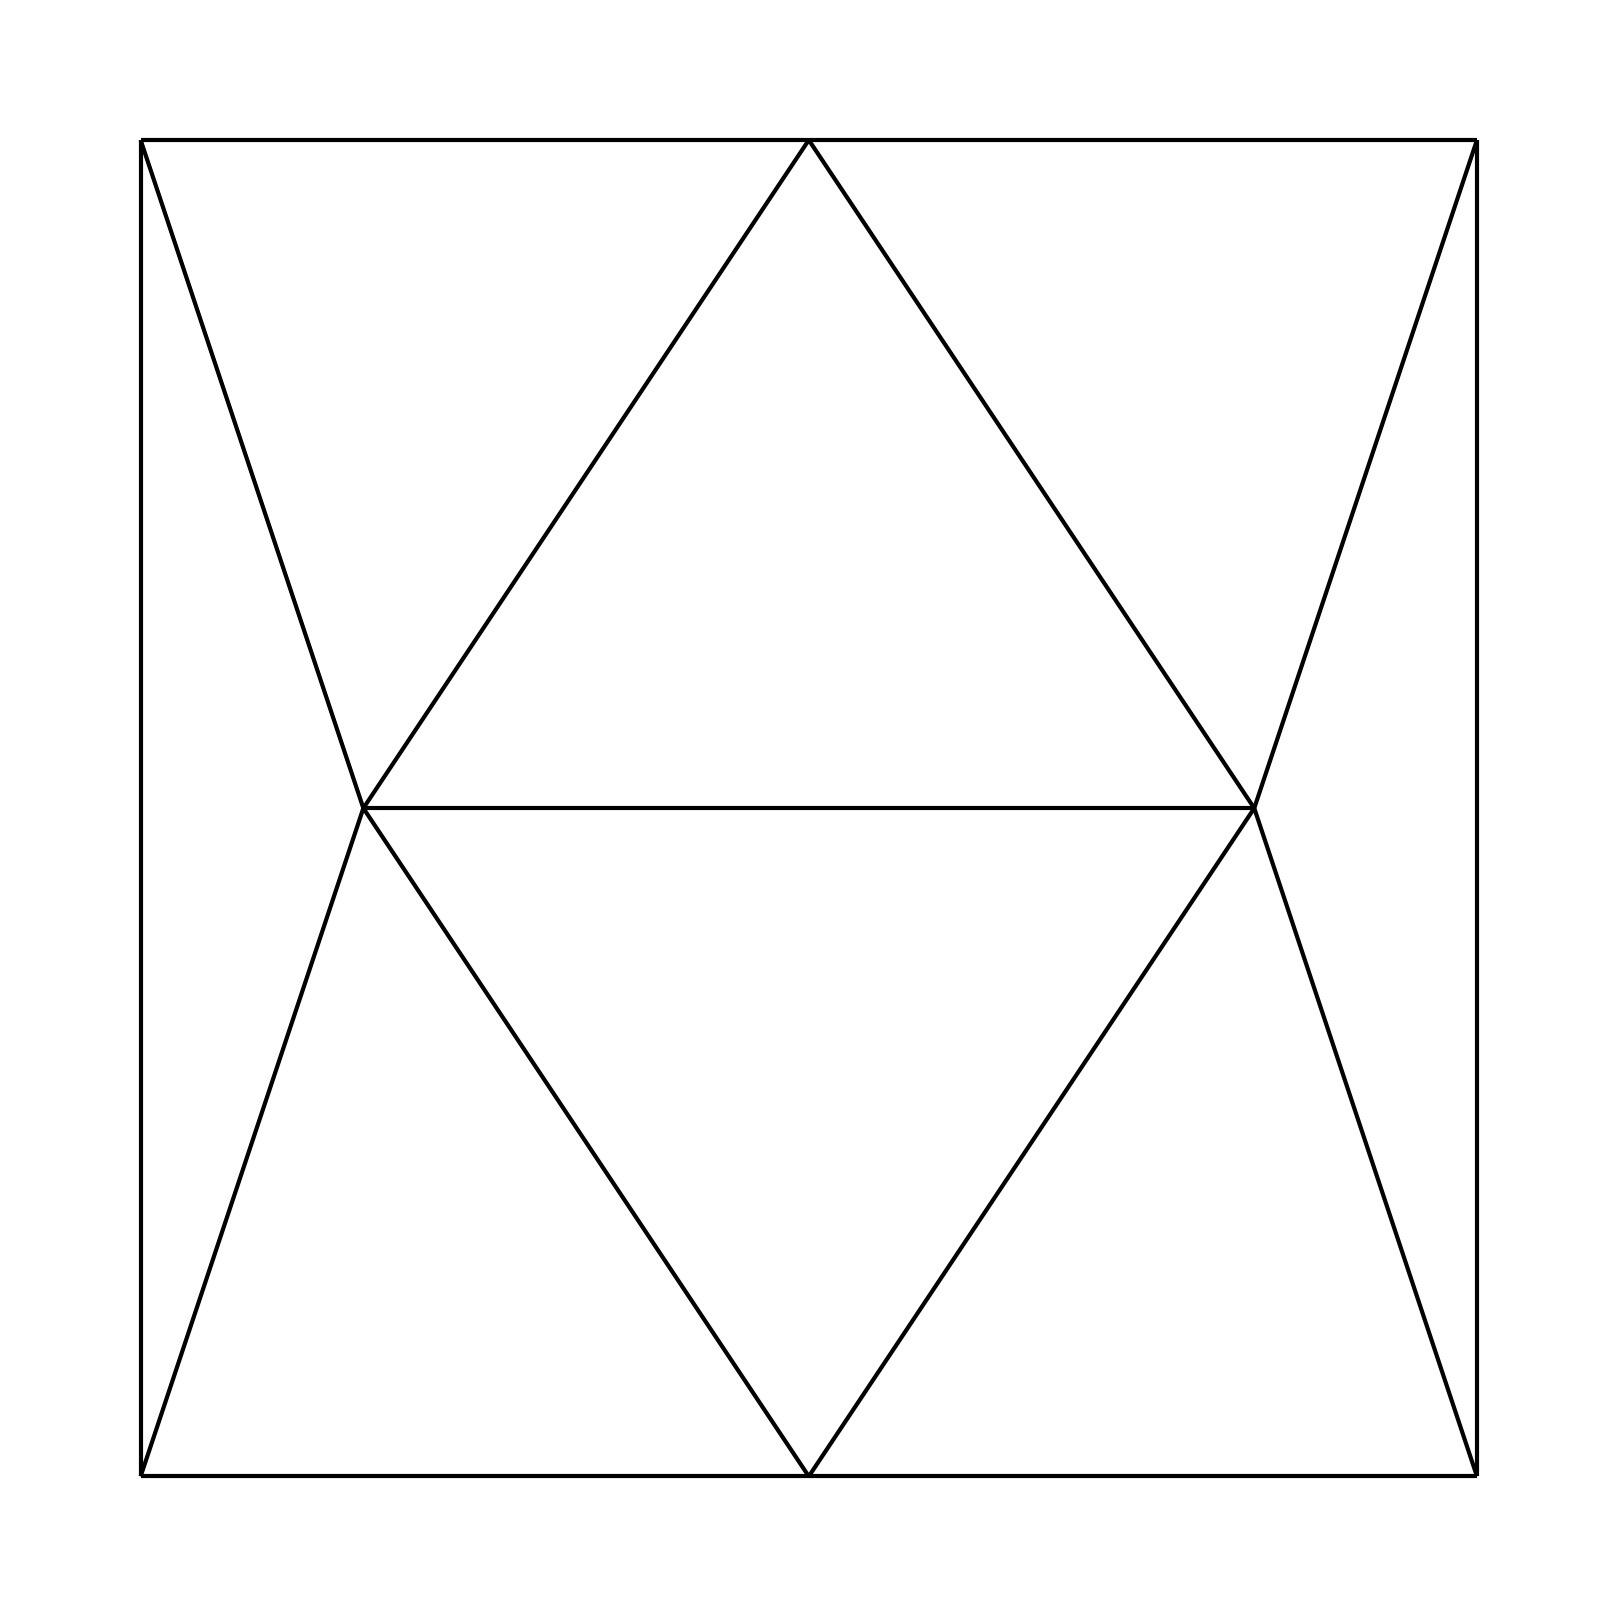
\includegraphics[width=0.75\columnwidth]{../images/bell_before_refinement.png}
    \captionof{figure}{Input mesh.}
    \label{fig:bell_input}
    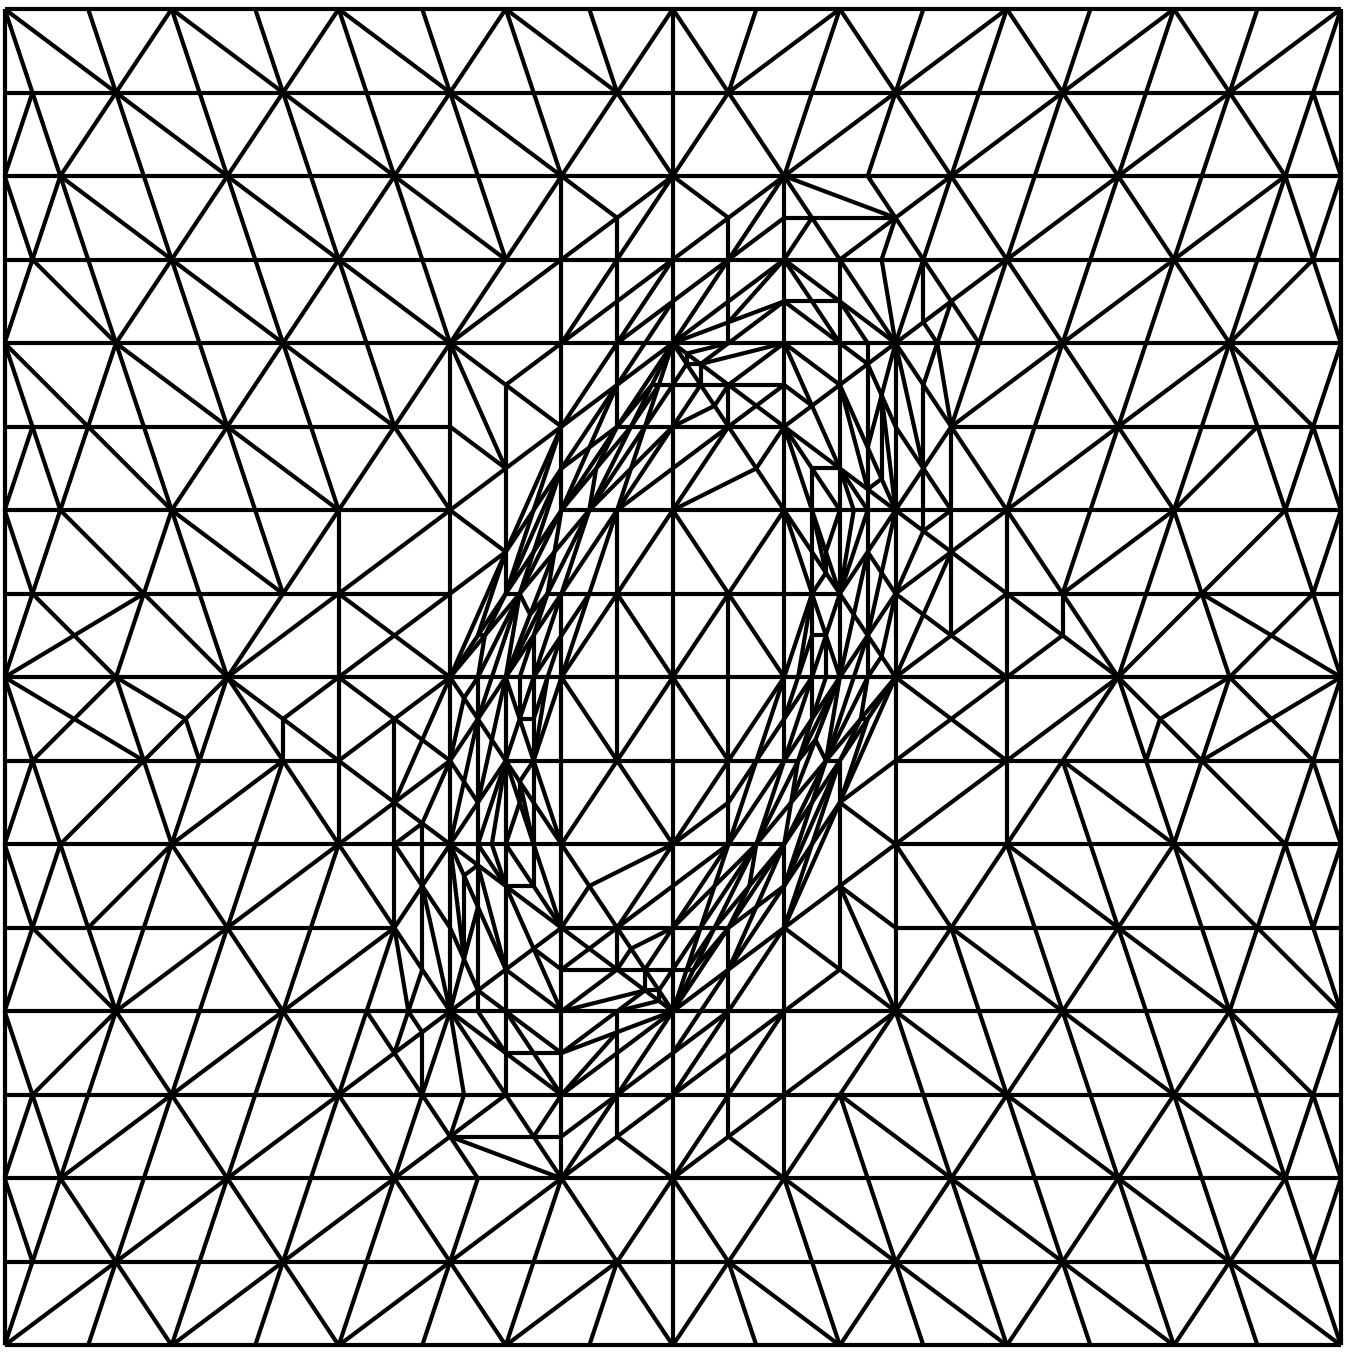
\includegraphics[width=0.75\columnwidth]{../images/bell_after_refinement.png}
    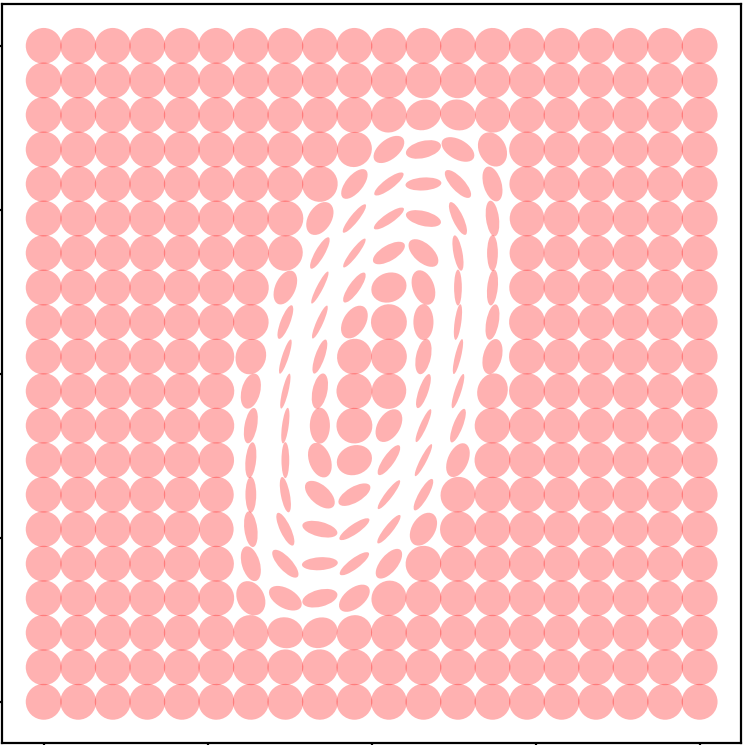
\includegraphics[width=0.75\columnwidth]{../images/bell_tissot.png}
    \captionof{figure}{Output mesh and Tissot's Indicatrices.}
    \label{fig:bell_tissot}
    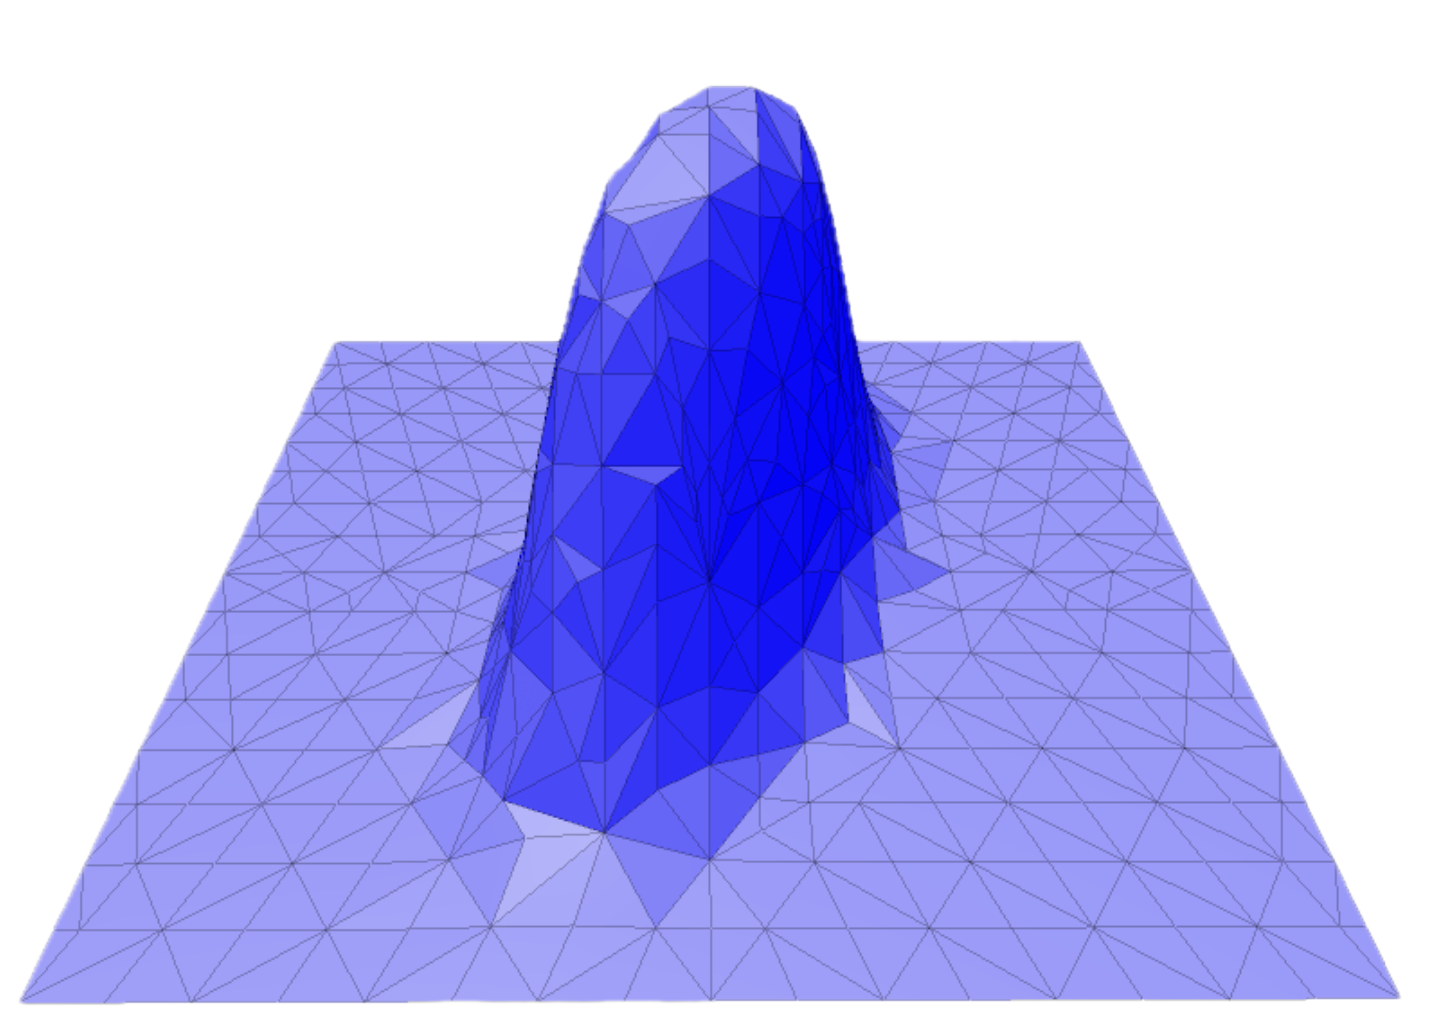
\includegraphics[width=0.94\columnwidth]{../images/bell_embedded.png}
    \captionof{figure}{Mapping the refined mesh through the embedding function $f$.}
    \label{fig:bell_embedded}
\end{figure}

\subsubsection*{Triangulating subset of the Hyperbolic Plane}
    We showcase the algorithm on the Poincaré disc model of $\mathbb{H}^2$ and compare with a hyperbolic tiling. As discussed in an earlier section, we cannot triangulate an unbounded domain, so we truncate the unit disc and look only within the disc of radius $0.97$. Algorithm run for $500$ steps with $A_{\text{max}} = \infty$ and $\rho = 1.9$. Setting $A_{\text{max}} = \infty$ leads to the parameter being ignored, while a high setting of $\rho$ makes the refinement phase focus just on making planar triangles, which means that all initial iterations are likely to focus on non-planar triangles only. 
    \\
    Figure \ref{fig:hyper_before} shows the input mesh $\mathbf{\Delta}_0$, which covers the $0.97$-disc somewhat uniformly. Three triangles on the way to the border have their edge-lengths marked. This is the length under the hyperbolic metric. The outermost triangle does not satisfy the triangle inequality in this initial mesh, as $1.34 + 2.04 < 6.08$. Figure \ref{fig:hyper_after} shows the output of the algorithm, an intrinsic triangulation of a subset of $\mathbb{H}^2$. The high triangle density at the edges highlights the hyperbolic expansion of space, which necessitates triangle subdivision. All triangles are congruent. The triangles in our tiling are not congruent and will depend on the initial triangulation, but $A_{\text{max}}$ ensures that we make splits around the edge proportional to the area. A common visualization of the hyperbolic plane is given in fig \ref{fig:hyper_tiling}, in which all triangles are congruent. This visualization bears resemblance to the one obtained in figure \ref{fig:hyper_after} and illustrates the hyperbolic expansion of space which necessitates triangle subdivision.
    \\
    \begin{figure}
        \centering
        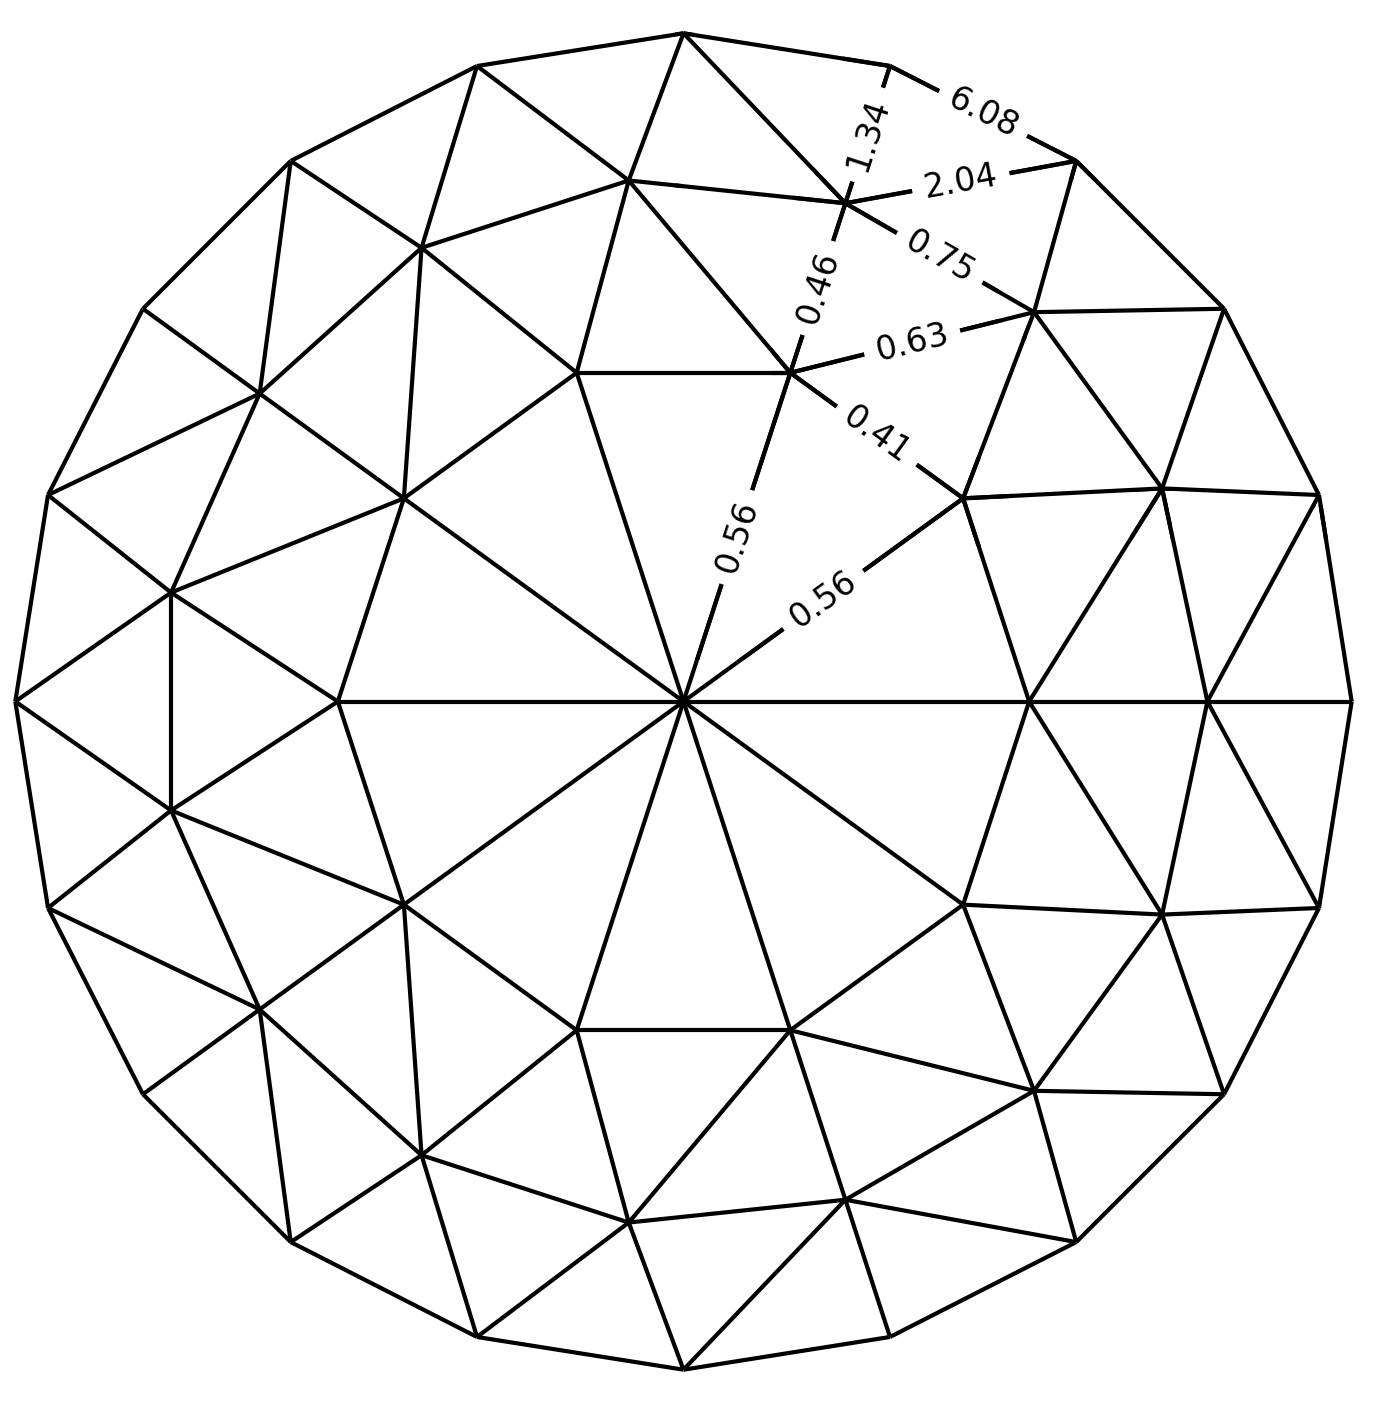
\includegraphics[width=0.85\columnwidth]{../images/hyperbolic_disc_before_refinement_some_labels.png}
        \captionof{figure}{Input mesh.}
        \label{fig:hyper_before}
        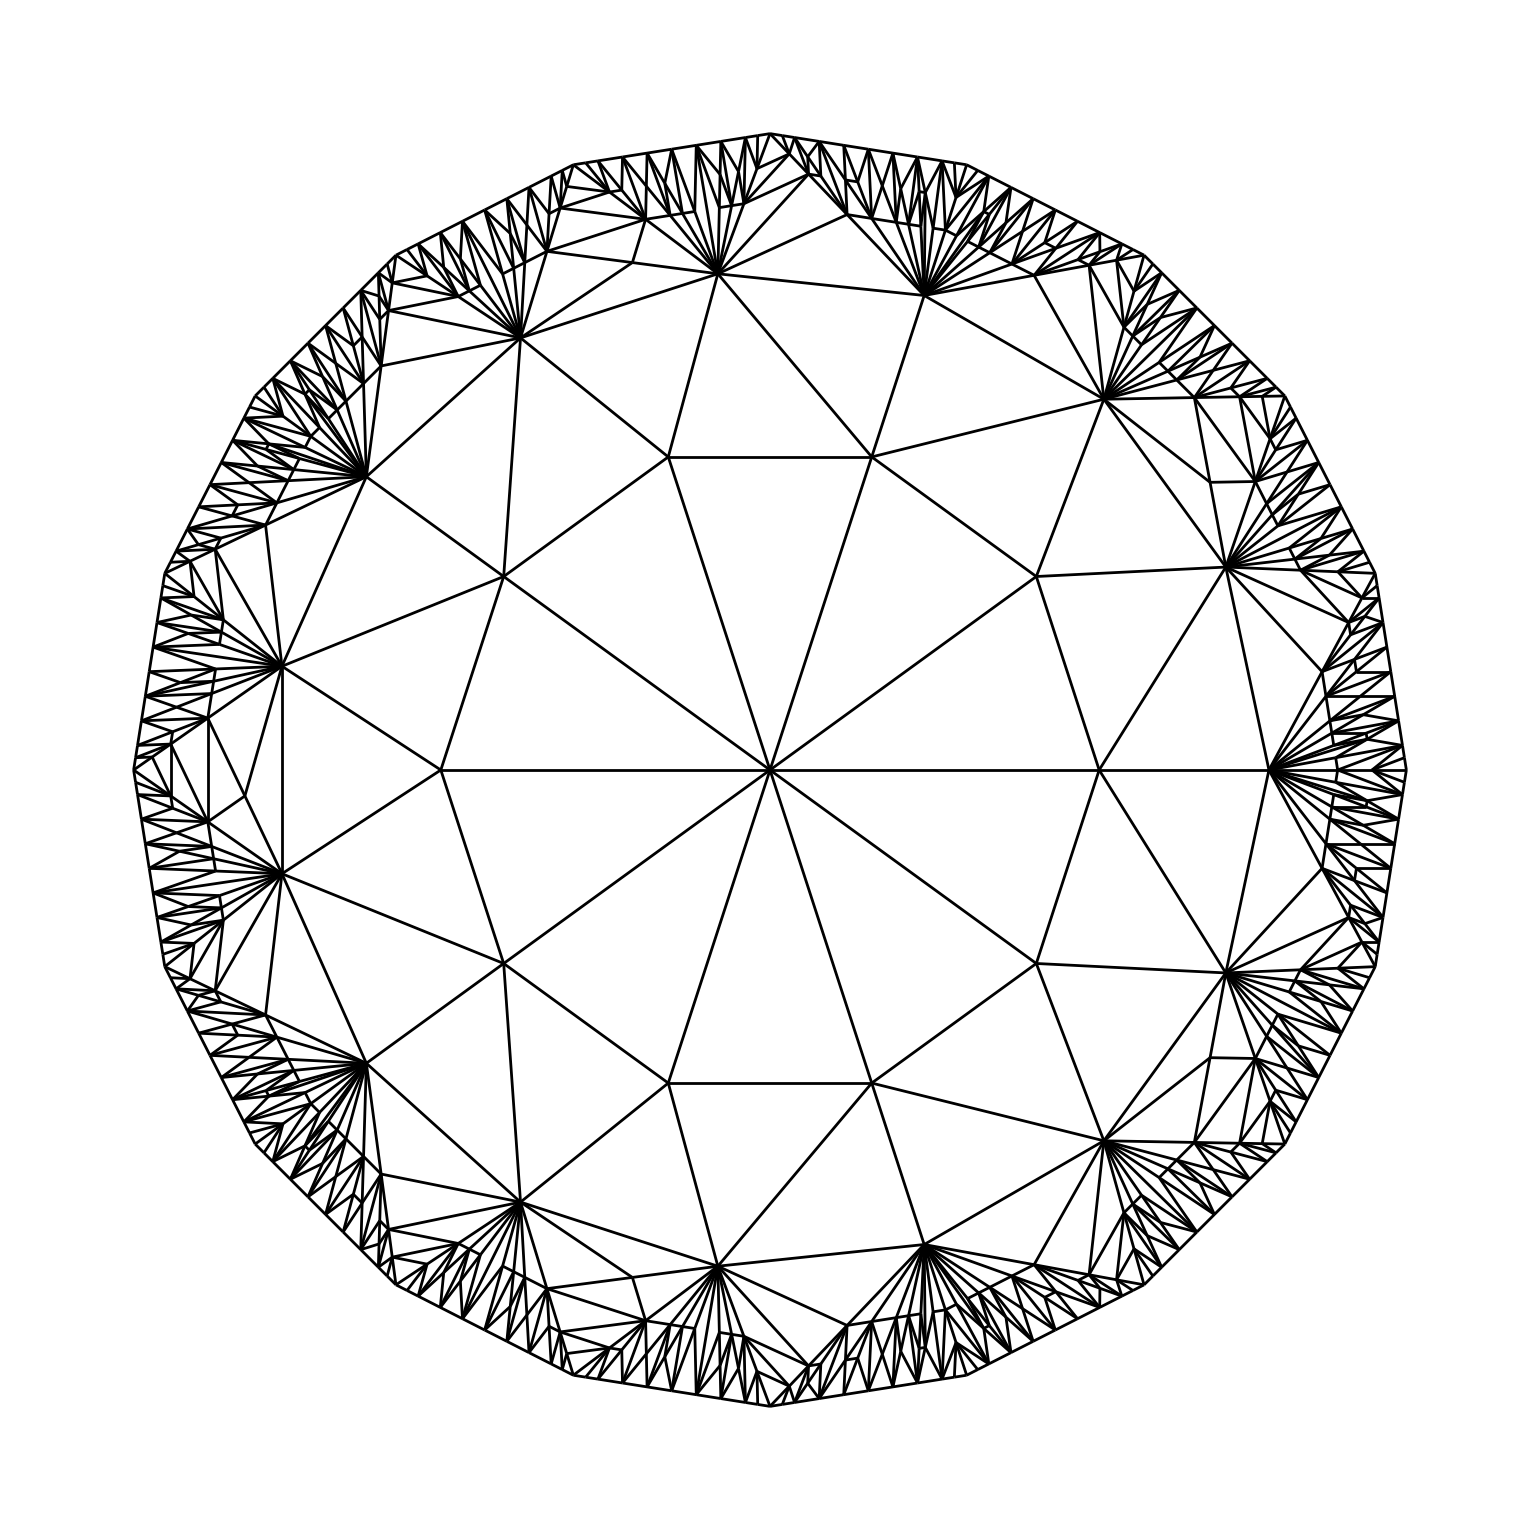
\includegraphics[width=0.85\columnwidth]{../images/hyperbolic_disc_after_refinement.png}
        \captionof{figure}{Output mesh}
        \label{fig:hyper_after}
        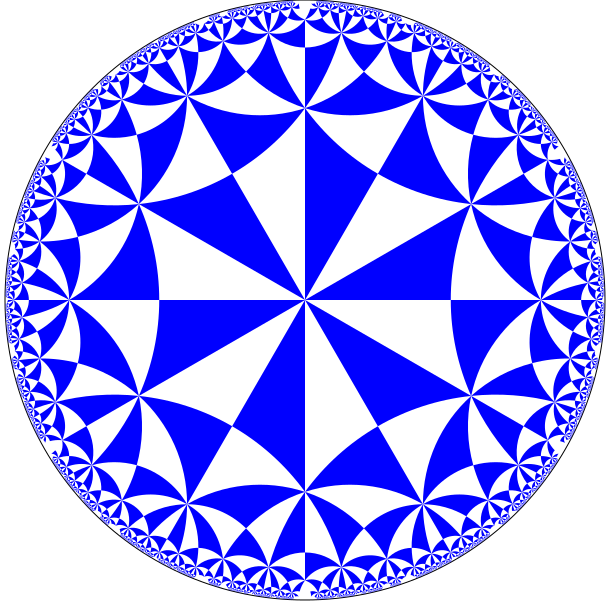
\includegraphics[width=0.85\columnwidth]{../images/wiki_hyperbolic.png}
        \captionof{figure}{Tiling of the hyperbolic plane from \cite{HyperbolicTiling}.}
        \label{fig:hyper_tiling}
        
    \end{figure}

\subsection*{Potential Improvements}
The metric tensor will be evaluated in the same vertex many times if the edge is split multiple times. One could cache the metric tensor at each vertex to avoid redundant computations.
\\\\
One could, assuming the fan-model, also compute the distance from the midpoint of the longest edge to the opposing corner as $(1 + 1.5) / 2 = 1.25$. Under that assumption it will yield exact distances. This could be done as the last split in each triangle so the approximation error does not propagate.
\\ An alternative approximation is that the metric will changes linearly between the two points of an edge. In this case the metric tensor must be computed only at the endpoints. With caching, one would have to compute it only once per vertex.
\\\\ Additionally, instead of bisecting the longest edge at its Euclidean midpoint (in coordinate space), one can run an incremental search along it to determine the midpoint in coordinate space under the metric $g$. This which would be a more reasonable choice for the new vertex and might save a few subdivisions. It can even be done at the same cost of the current algorithm, since, once the midpoint is found, one will know that the lengths of the two constituent edges are equal and sum to the original length.
\\\\ After the refinement phase, one can run edge-flipping (\cite{sharp2021intrinsic}, \cite{intrinsic_laplacian}) to further improve the quality. This is an operation applicable to intrinsic triangulations that swaps diagonal edges of a quadrilateral if it improves the quality of the triangulation.
\\\\ Alternatively to edge-flipping, one could use a different subdivision scheme, such as red-green refinement. This is more complex, but might yield better results as it is free to place new vertices in the interior of the triangle, not just on the edges.
\\\\ Generally, the greedy subdivision scheme could be improved upon or replaced. If one zooms in on the picture in figure \ref{fig:bell_embedded}, one notices a so-called "rat-nest", which is a vertex with many incident edges. This is a common problem in greedy subdivision schemes, and will generally lead to elongated triangles. The bisection method can never get rid of a rat-nest after it has made one.
\\\\
\subsection*{Experiment with the Laplacian}
We will perform an experiment with the Laplacian of this mesh in chapter \ref{sec:solver_experiments}, after having defined the probabilistic numerical solver in the following two chapters.
\ifdefined\COMPILINGFROMMAIN
\else
    \end{document}
\fi